\chapter{HASIL DAN PEMBAHASAN}
Pada penelitian ini dipaparkan hasil penelitian serta analisis dari model klasifikasi yang telah dibuat sesuai dengan desain sistem dan implementasi pada Bab 3. Data yang digunakan pada pengujian ini menggunakan dataset DRAC dengan data splitting yang telah dilakukan pra-pemrosesan sebelumnya.
\section{Hasil Penelitian}

\section{Hasil Pengujian}
\subsection{Hasil pengujian Model tanpa menggunakan penyesuaian apapun}
    \begin{figure}[H]
        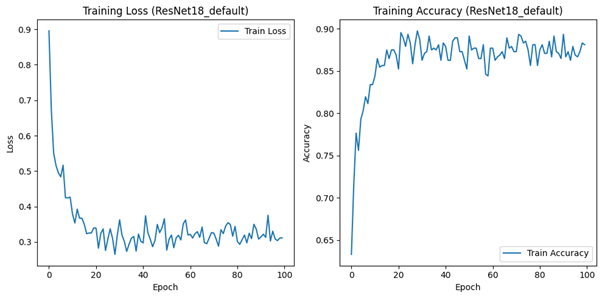
\includegraphics[scale=0.8]{gambar/TrainingGraphResNet18.png}
        \caption{Training Loss dan Akurasi ResNet-18}
        \label{Img:GraphResNet18}
    \end{figure}
    \begin{figure}[H]
        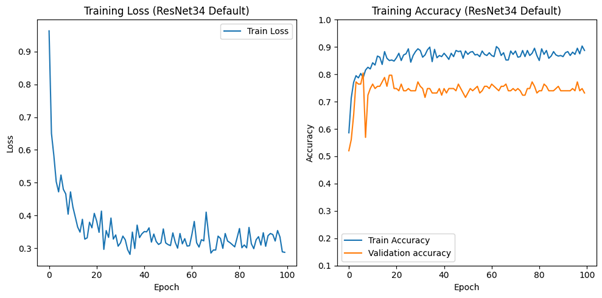
\includegraphics[scale=0.8]{gambar/TrainingGraphResNet34.png}
        \caption{Training Loss dan Akurasi ResNet-34}
        \label{Img:GraphResNet34}
    \end{figure}
    \begin{figure}[H]
        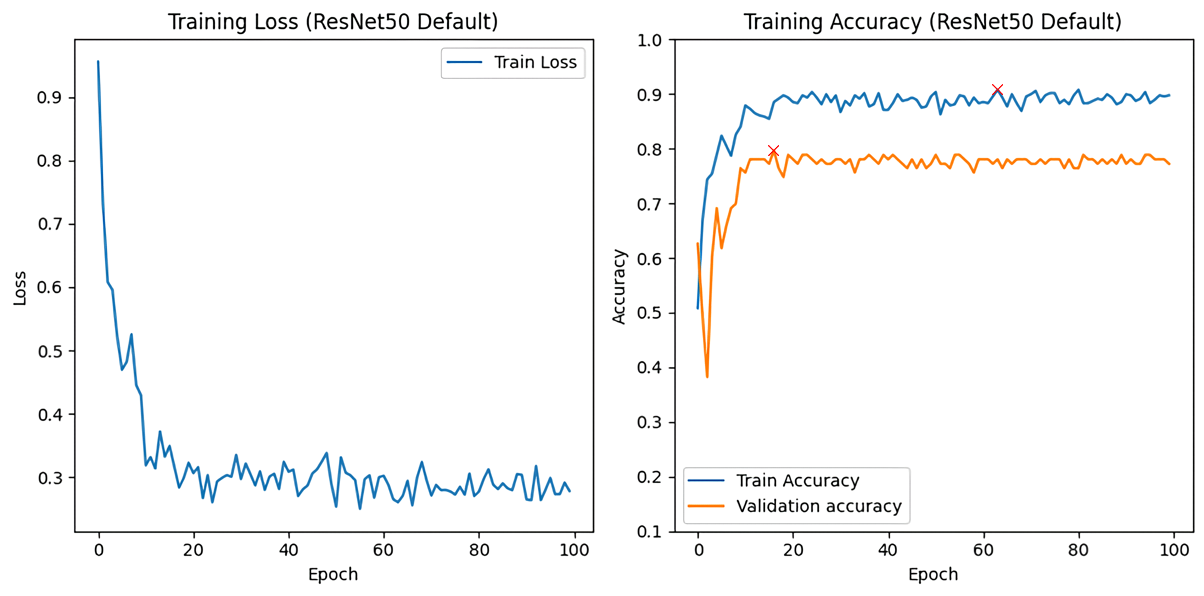
\includegraphics[scale=0.8]{gambar/TrainingGraphResNet50.png}
        \caption{Training Loss dan Akurasi ResNet-50}
        \label{Img:GraphResNet50}
    \end{figure}
    \begin{figure}[H]
        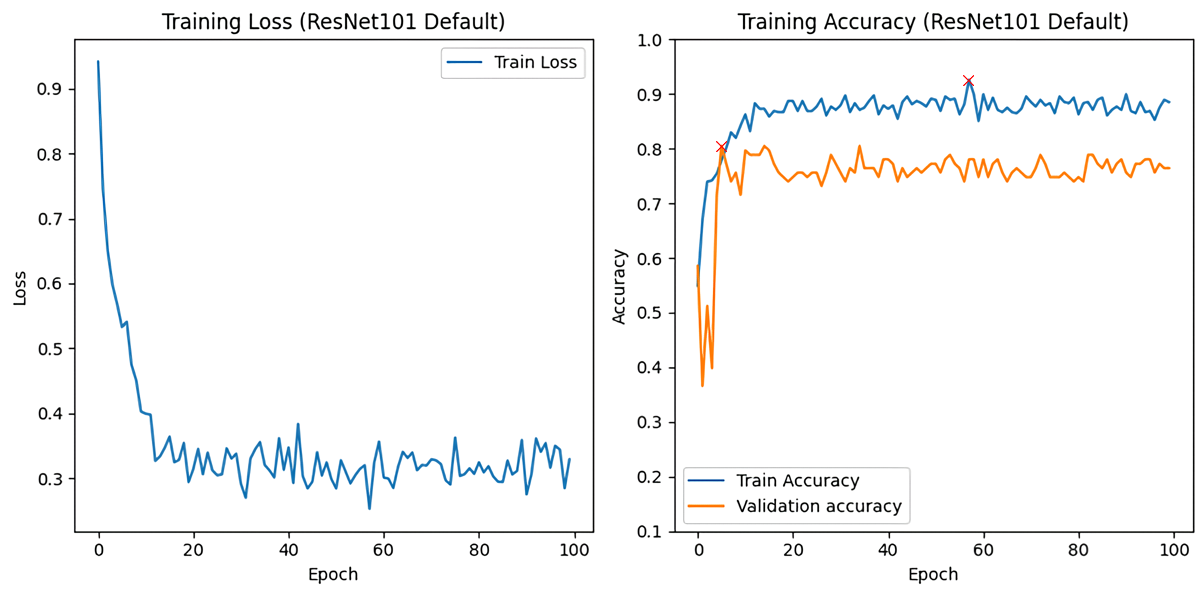
\includegraphics[scale=0.8]{gambar/TrainingGraphResNet101.png}
        \caption{Training Loss dan Akurasi ResNet-101}
        \label{Img:GraphResNet101}
    \end{figure}
    \begin{figure}[H]
        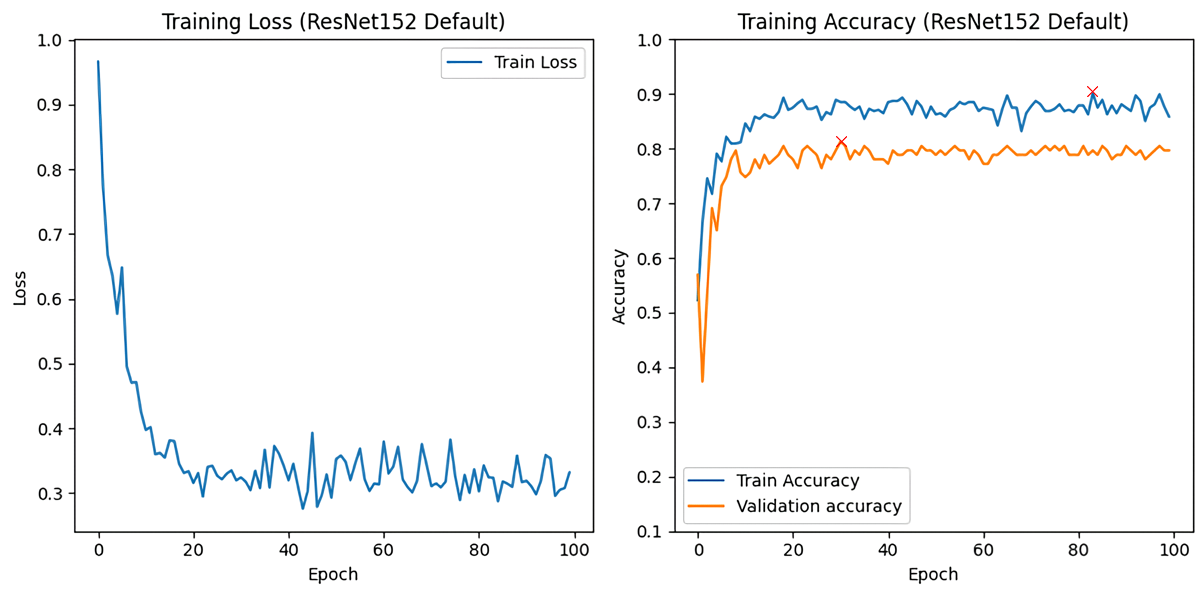
\includegraphics[scale=0.8]{gambar/TrainingGraphResNet152.png}
        \caption{Training Loss dan Akurasi ResNet-152}
        \label{Img:GraphResNet152}
    \end{figure}

    \begin{table}[H]
        \begin{center}
        \caption{Hasil training best model tanpa melalui penyesuaian class dataset}
        \label{tb:HasilTrainClassWeight}
            \begin{tabular}{clclll}
            \cline{1-6}
            ResNet   architecture & \multicolumn{1}{c}{class} & acc                     & \multicolumn{1}{c}{prec} & \multicolumn{1}{c}{rec} & \multicolumn{1}{c}{F1} \\ \cline{1-6}
            \multirow{3}{*}{18}   & non-DR                    & \multirow{3}{*}{0,7642} & 0,861538                 & 0,848485                & 0,854962               \\
                                  & NPDR                      &                         & 0,652174                 & 0,697674                & 0,674157               \\
                                  & PDR                       &                         & 0,666667                 & 0,571429                & 0,615385               \\ \cline{1-6}
            \multirow{3}{*}{34}   & non-DR                    & \multirow{3}{*}{0,7724} & 0,857143                 & 0,818182                & 0,837209               \\
                                  & NPDR                      &                         & 0,666667                 & 0,790698                & 0,723404               \\
                                  & PDR                       &                         & 0,777778                 & 0,5                     & 0,608696               \\ \cline{1-6}
            \multirow{3}{*}{50}   & non-DR                    & \multirow{3}{*}{0,6992} & 0,808824                 & 0,833333                & 0,820896               \\
                                  & NPDR                      &                         & 0,581395                 & 0,581395                & 0,581395               \\
                                  & PDR                       &                         & 0,5                      & 0,428571                & 0,461538               \\ \cline{1-6}
            \multirow{3}{*}{101}  & non-DR                    & \multirow{3}{*}{0,8049} & 0,909091                 & 0,909091                & 0,909091               \\
                                  & NPDR                      &                         & 0,711111                 & 0,744186                & 0,727273               \\ 
                                  & PDR                       &                         & 0,583333                 & 0,5                     & 0,538462               \\ \cline{1-6}
            \multirow{3}{*}{152}  & non-DR                    & \multirow{3}{*}{0,7398} & 0,852459                 & 0,787879                & 0,818898               \\
                                  & NPDR                      &                         & 0,603774                 & 0,744186                & 0,666667               \\
                                  & PDR                       &                         & 0,777778                 & 0,5                     & 0,608696               \\ \cline{1-6}
            \end{tabular}
        \end{center}
    \end{table}


\subsection{Hasil Pengujian Model dengan penyesuaian menggunakan class-weight}

    \begin{figure}[H]
        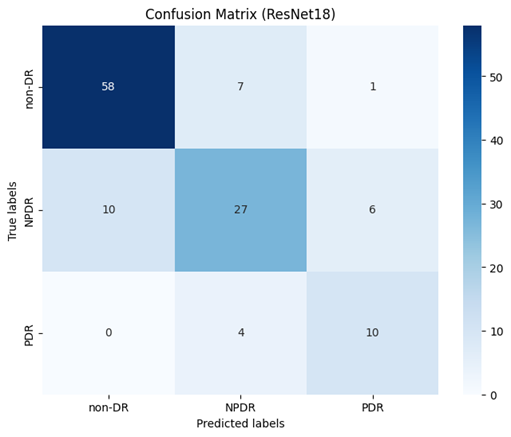
\includegraphics[scale=0.75]{gambar/confusionMatrixResnet18class-weighted.png}
        \caption{Training Loss dan Akurasi ResNet18}
        \label{fig:GraphResNet18class}
    \end{figure}

    \begin{table}[h!]
        \begin{center}
        \caption{Hasil training best model menggunakan class-weight adjustment}
        \label{tb:HasilTrainClassWeight}
            \begin{tabular}{clclll}
            \cline{1-6}
            ResNet   architecture & \multicolumn{1}{c}{class} & acc                     & \multicolumn{1}{c}{prec} & \multicolumn{1}{c}{rec} & \multicolumn{1}{c}{F1} \\ \cline{1-6}
            \multirow{3}{*}{18}   & non-DR                    & \multirow{3}{*}{0,7724} & 0,852941                 & 0,878788                & 0,865672               \\
                                  & NPDR                      &                         & 0,710526                 & 0,627907                & 0,666667               \\
                                  & PDR                       &                         & 0,588235                 & 0,714286                & 0,645161               \\ \cline{1-6}
            \multirow{3}{*}{34}   & non-DR                    & \multirow{3}{*}{0,748}  & 0,857143                 & 0,818182                & 0,837209               \\
                                  & NPDR                      &                         & 0,652174                 & 0,697674                & 0,674157               \\
                                  & PDR                       &                         & 0,571429                 & 0,571429                & 0,571429               \\ \cline{1-6}
            \multirow{3}{*}{50}   & non-DR                    & \multirow{3}{*}{0,7236} & 0,822581                 & 0,772727                & 0,796875               \\
                                  & NPDR                      &                         & 0,608696                 & 0,651163                & 0,629213               \\
                                  & PDR                       &                         & 0,666667                 & 0,714286                & 0,689655               \\ \cline{1-6}
            \multirow{3}{*}{101}  & non-DR                    & \multirow{3}{*}{0,7724} & 0,901639                 & 0,833333                & 0,866142               \\
                                  & NPDR                      &                         & 0,666667                 & 0,697674                & 0,681818               \\
                                  & PDR                       &                         & 0,588235                 & 0,714286                & 0,645161               \\ \cline{1-6}
            \multirow{3}{*}{152}  & non-DR                    & \multirow{3}{*}{0,7154} & 0,892857                 & 0,757576                & 0,819672               \\
                                  & NPDR                      &                         & 0,604167                 & 0,674419                & 0,637363               \\
                                  & PDR                       &                         & 0,473684                 & 0,642857                & 0,545455               \\ \cline{1-6}
            \end{tabular}
        \end{center}
    \end{table}